\documentclass[10pt]{article}
\usepackage[a4paper, margin=2.3cm]{geometry}
\usepackage{titlesec}
\usepackage{graphicx}
\usepackage{subcaption}
\usepackage{booktabs}
\usepackage{amsmath}
\usepackage{hyperref}
\usepackage{enumitem}
\usepackage{parskip}
\usepackage{xcolor}
\usepackage{ulem}
\usepackage{float}
\usepackage{placeins}
\usepackage{tikz}
\usepackage{caption}
\usetikzlibrary{arrows.meta}

% Compact formatting to keep the report within the 8-page limit
\linespread{0.98}
\setlength{\textfloatsep}{6pt plus 1pt minus 1pt}
\setlength{\floatsep}{5pt plus 1pt minus 1pt}
\setlength{\intextsep}{5pt plus 1pt minus 1pt}
\setlength{\abovecaptionskip}{3pt}
\setlength{\belowcaptionskip}{1pt}
\setlength{\parskip}{3pt}
\setlist[itemize]{noitemsep, topsep=0pt, parsep=0pt, partopsep=0pt}
\urlstyle{same}
\def\UrlBreaks{\do\/\do-\do\_}

\definecolor{figBlue}{HTML}{2563EB}
\definecolor{figGreen}{HTML}{16A34A}
\definecolor{figAmber}{HTML}{D97706}
\definecolor{figPink}{HTML}{DB2777}
\definecolor{figIndigo}{HTML}{4F46E5}
\definecolor{figCyan}{HTML}{0284C7}
\definecolor{figOrange}{HTML}{EA580C}
\definecolor{figRed}{HTML}{DC2626}
\definecolor{figOlive}{HTML}{65A30D}
\captionsetup{font=small}

\title{COMP3242 Group Project Report\\Ablation Study of SimCLR Components}

\titleformat{\section}
  {\normalfont\large\bfseries}
  {\thesection}
  {0.8em}
  {}

\titleformat{\subsection}
  {\normalfont\normalsize\bfseries}
  {\thesubsection}
  {0.8em}
  {}

\titlespacing*{\section}{0pt}{8pt}{8pt}
\titlespacing*{\subsection}{0pt}{7pt}{6pt}

\author{
Chengbo Yan \\ \texttt{u7515796}
\and
Guochen Wang \\ \texttt{u7663394}
\and
Weiyi Jiang \\ \texttt{u8191809}
}

\date{June 2026}

\begin{document}

\maketitle

\section*{Declaration of Originality}

We, \underline{Chengbo Yan} (UID: \underline{u7515796}), \underline{Weiyi Jiang} (UID: \underline{u8191809}), and \underline{Guochen Wang} (UID: \underline{u7663394}), here declare that the report, experimental design, modifications, experiments, analysis, and submitted results are our own work. Our implementation is adapted from the open-source \texttt{sthalles/SimCLR} PyTorch repository~\cite{sthalles_simclr}, with our own modifications for ablation experiments, low-label evaluation, large-batch learning-rate follow-up, result visualization, and analysis.

\vspace{0.8em}

We confirm that we have not copied text, results, or unacknowledged code from other students or external sources. External code used as a starting point is explicitly acknowledged and cited. We understand that plagiarism or any form of academic dishonesty is not permitted.

\vspace{0.8em}

\textbf{AI Use: In completing this assignment, we declare that we:}

\fbox{\rule{0pt}{1.1ex}\rule{1.1ex}{0pt}}~\textbf{Have not used any AI tools}

\fbox{\scriptsize X}~\textbf{Have used AI tools} (e.g., ChatGPT, DeepSeek, or similar AI systems)

\vspace{0.8em}

Description of AI use: \uline{We used AI as a support tool for debugging discussion, concept explanation, report organisation, language editing, and wording polishing. AI was not used to generate final experimental results. The final implementation, testing, design decisions, report wording, code comments, and submitted results were checked, revised, and accepted by our group. To verify the correctness of our implementation, we tested the program on multiple cases and confirmed that the outputs matched the expected results. In addition, all group members reviewed the code and results carefully to ensure all contents worked as intended.}

\vspace{0.8em}

\textbf{Short statement on individual contributions:}
\begin{itemize}[leftmargin=1.5em]
    \item Chengbo Yan (u7515796): \uline{low-label evaluation, non-frozen transfer comparison, large-batch learning-rate follow-up, result analysis, and report writing.}
    \item Guochen Wang (u7663394): \uline{projection head ablation, batch size ablation, result visualization and analysis, and report writing.}
    \item Weiyi Jiang (u8191809): \uline{data augmentation ablation, comparison of baseline, no\_blur, no\_color\_jitter, and no\_grayscale settings, result visualization, and analysis.}
\end{itemize}

\vspace{1em}

\begin{abstract}
This report presents a controlled ablation study of SimCLR on CIFAR-10 using a ResNet-18 encoder. We evaluate how data augmentation, projection head design, batch size, and label availability affect downstream representation quality, using frozen linear evaluation as the main metric. Removing ColorJitter causes the largest drop in linear evaluation accuracy, from 68.20\% to 62.61\%, while removing Gaussian blur has little effect. The projection head gives a modest improvement, increasing best accuracy from 62.16\% to 63.59\%. Batch size 256 performs best under the default setup, but batch size 1024 recovers from 57.56\% to 65.43\% after learning-rate tuning. Low-label experiments show that SimCLR mainly improves label efficiency. Overall, SimCLR performance in this lightweight setting depends on both representation design and optimization matching.
\end{abstract}

\newpage
\section{Introduction}

Deep neural networks usually require large labeled datasets to learn useful visual representations. However, collecting such labels in the real world is often expensive, time consuming, and difficult. Self-supervised learning reduces this dependence by learning representations from unlabeled data and evaluating whether the learned features transfer to downstream tasks.

This report studies SimCLR, a contrastive self-supervised learning framework for visual representation learning~\cite{simclr}. SimCLR trains an encoder using two augmented views of each image as a positive pair, while treating other images in the batch as negatives. After pretraining, we use frozen linear evaluation to measure representation quality.

We conduct a controlled empirical study of SimCLR on CIFAR-10 with a ResNet-18 encoder. Our experiments examine data augmentation, projection head design, batch size, low-label transfer, and large-batch learning-rate tuning. Overall, the results show that SimCLR performance depends on both representation design and optimization details.

\section{Background and Related Work}

SimCLR is a contrastive self-supervised learning framework for visual representation learning~\cite{simclr}. It learns representations by generating two augmented views of each image, treating them as a positive pair, and contrasting them against other images in the same batch using the NT-Xent loss. Earlier contrastive methods use related objectives: Contrastive Predictive Coding (CPC) identifies positive samples among negatives in latent space~\cite{cpc}, while MoCo uses a momentum encoder and a queue of negative examples to build a large dictionary for contrastive learning~\cite{moco}. Compared with these methods, SimCLR removes the memory bank and momentum encoder, relying instead on strong data augmentation, a nonlinear projection head, large batch sizes, and the NT-Xent loss~\cite{simclr}.

Our work focuses on SimCLR because these design choices directly match our ablation questions. The original SimCLR study shows that data augmentation, the nonlinear projection head, batch size, and training steps are important for contrastive representation learning~\cite{simclr}. However, these findings are mainly established in larger-scale settings. We therefore analyse these components in a smaller CIFAR-10 setting, where limited image resolution, fewer semantic classes, and constrained computation may change how these components behave.

Data augmentation is central to contrastive learning because it defines what information should be invariant across two views of the same image. Tian et al.~\cite{goodviews} argue that effective views should remove task-irrelevant information while preserving task-relevant information. This motivates our augmentation ablation. In particular, color information can become a low-level shortcut: without sufficient color perturbation, the model may match positive pairs using similar color statistics rather than learning more transferable semantic features. Therefore, we test the effect of removing Gaussian blur, random grayscale, and ColorJitter on downstream representation quality.

The projection head and batch size are related to how the contrastive loss shapes the representation space. Wang and Isola~\cite{alignuniform} describe contrastive learning in terms of alignment and uniformity: positive pairs should be close, while representations should remain spread out across the feature space. In SimCLR, a larger batch provides more in-batch negatives, which may help the uniformity objective. However, larger batches also change other factors at the same time. Under a fixed number of epochs, they receive fewer optimizer updates, and on CIFAR-10 they may increase the chance that same-class images are treated as negatives. This trade-off motivates our batch-size ablation and the large-batch learning-rate follow-up.

Low-label evaluation tests whether self-supervised representations reduce dependence on labeled data. SimCLRv2 shows that self-supervised pretraining is especially useful in semi-supervised and low-label settings~\cite{simclrv2}, while supervised contrastive learning shows that contrastive objectives remain useful when label information is available~\cite{supcon}. These works motivate our comparison between frozen linear evaluation, SimCLR fine-tuning, and supervised training from scratch under limited labels.

\section{Methods}

\subsection{Implementation Overview}

Our implementation follows the full SimCLR workflow: generating two augmented views per image, training a ResNet-18 encoder with the NT-Xent loss, extracting frozen encoder features, and training a linear classifier for downstream evaluation. This modular structure allows each ablation to modify one component while keeping the rest of the pipeline fixed.

\subsection{Baseline SimCLR Pipeline}

Our baseline follows the standard SimCLR pretraining and linear evaluation pipeline~\cite{simclr}. We use CIFAR-10~\cite{cifar10} as the dataset and ResNet-18~\cite{resnet} as the encoder backbone. During contrastive pretraining, each input image is transformed twice to produce two augmented views. The augmentation pipeline includes random resized crop, horizontal flip, color jitter, random grayscale, and Gaussian blur. For a batch of $B$ original images, the model receives $2B$ augmented views. For each anchor view, the positive example is the other view generated from the same original image, while the remaining $2(B-1)$ views are treated as negatives.

The contrastive loss follows the normalized temperature-scaled cross entropy loss used by SimCLR:
\[
\ell_{i,j} =
-\log
\frac{\exp(\operatorname{sim}(z_i,z_j)/\tau)}
{\sum_{k=1}^{2B} \mathbf{1}_{k \ne i}
\exp(\operatorname{sim}(z_i,z_k)/\tau)} ,
\]
where $z$ is the normalized representation used by the contrastive loss, $\operatorname{sim}$ is cosine similarity, and $\tau$ is the temperature. In our experiments, the temperature is set to 0.07. Unless otherwise stated, pretraining uses 100 epochs and Adam optimization.

\subsection{Projection Head and Encoder Representation}

The ResNet-18 encoder outputs a 512-dimensional feature vector $h$. With the projection head enabled, $h$ is passed through a two-layer multi-layer perceptron:
\[
512 \rightarrow 512 \rightarrow 128.
\]
The contrastive loss is applied to the projected vector $z$, while downstream evaluation uses the encoder feature $h$. In the no-projection-head ablation, the contrastive loss is applied directly to the 512-dimensional encoder output. This comparison tests whether separating the contrastive space from the downstream feature space improves representation quality.

\subsection{Linear Evaluation Protocol}

After SimCLR pretraining, the encoder is frozen and a single linear classifier is trained on extracted CIFAR-10 features for 100 epochs using Adam with learning rate 0.001 and no weight decay. Since the encoder is not updated, test accuracy mainly reflects the quality of the pretrained representation. The reported best accuracy is the highest test accuracy observed during the corresponding linear evaluation.

\subsection{Ablation Design}

We run controlled ablations by changing one factor at a time while keeping the dataset, backbone, and evaluation protocol fixed as much as possible. The main baseline checkpoint uses the full SimCLR augmentation pipeline and reaches 68.20\% frozen linear evaluation accuracy. Data augmentation, low-label evaluation, and large-batch learning-rate follow-up use this main baseline, while projection-head and batch-size experiments are interpreted within their own controlled ablation groups.

\section{Experiments and Results}

This section reports the main ablation results. Unless otherwise stated, results are compared against the main baseline with 68.20\% frozen linear evaluation accuracy. Projection-head and batch-size results are interpreted within their own controlled ablation groups.

\subsection{Data Augmentation Ablation}

To identify which augmentation component affects downstream representation quality most, we remove one component from the pipeline at a time while keeping other training settings fixed.

\begin{table}[H]
\centering
\small
\begin{tabular}{llcc}
\toprule
\textbf{Setting} & \textbf{Change from baseline} & \textbf{Contrastive Top-1} & \textbf{Linear eval acc. (\%)} \\
\midrule
baseline & Full augmentation pipeline & 60.45 & \textbf{68.20} \\
no\_blur & Remove Gaussian blur & 63.45 & 68.05 \\
no\_grayscale & Remove random grayscale & 69.18 & 65.23 \\
no\_color\_jitter & Remove ColorJitter & \textbf{82.00} & 62.61 \\
\bottomrule
\end{tabular}
\caption{Data augmentation ablation. The best contrastive pretraining metric does not correspond to the best downstream linear evaluation accuracy.}
\label{tab:augmentation}
\end{table}

\begin{figure}[H]
\centering
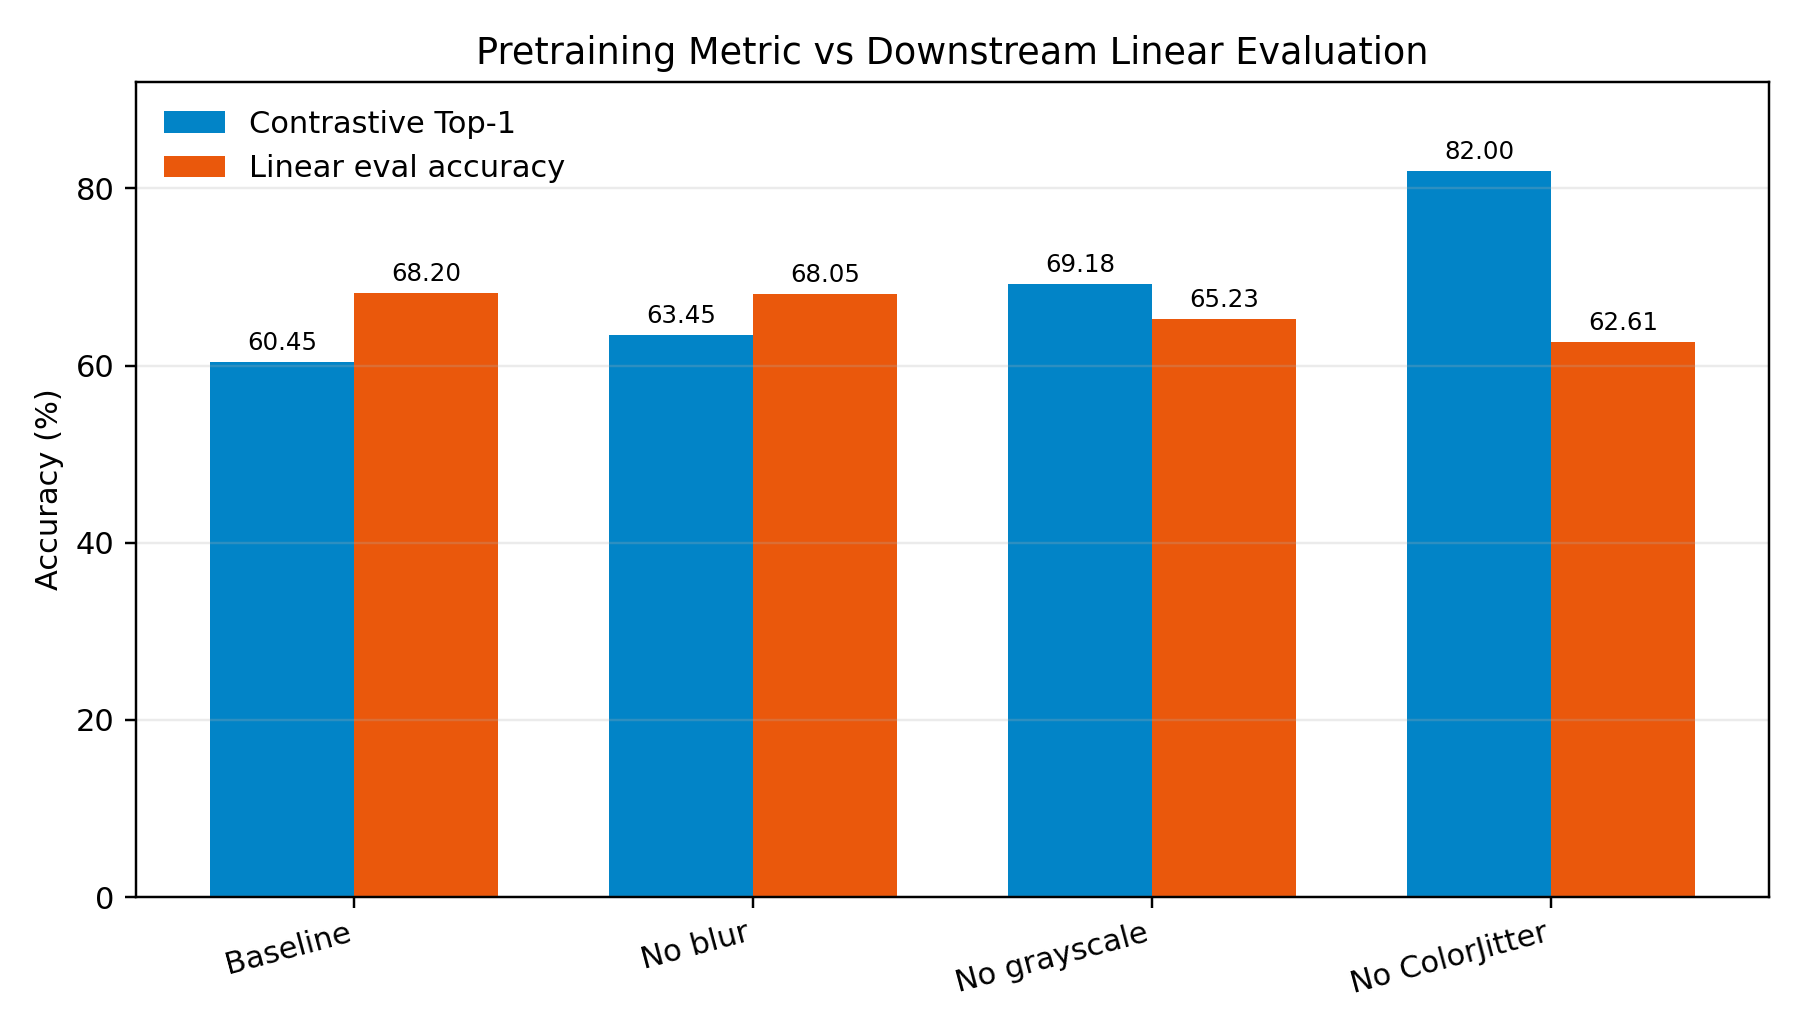
\includegraphics[width=0.70\textwidth]{augmentation_figures/augmentation_metrics_bar.png}
\caption{Visualization of the data augmentation ablation results.}
\label{fig:augmentation-visualization}
\end{figure}

The baseline obtains the best downstream accuracy. Removing Gaussian blur gives a nearly identical result, so we do not treat the small difference between 68.20\% and 68.05\% as meaningful. Removing random grayscale causes a larger drop, while removing ColorJitter gives the largest decline, suggesting that ColorJitter is the most important tested augmentation in our setting.

The contrastive Top-1 metric does not match the downstream ranking: the no\_color\_jitter setting has the highest contrastive Top-1 score but the worst linear evaluation accuracy. This suggests that a high pretraining score can reflect an easier pretext task rather than a better representation. Without ColorJitter, the model may use low-level color similarity to match positive pairs instead of learning more transferable semantic features.

\subsection{Projection Head Ablation}

We evaluate the projection head by comparing the standard SimCLR setting against a variant where the contrastive loss is applied directly to the 512-dimensional encoder output $h$. With the projection head, the model reaches 63.59\% best linear evaluation accuracy and 62.84\% final accuracy. Without the projection head, the best and final accuracies drop to 62.16\% and 61.40\%, respectively.

\begin{figure}[H]
\centering
\begin{subfigure}{0.45\textwidth}
    \centering
    
\includegraphics[width=\textwidth]{head_figures/accuracy_curve.png}
    \caption{Linear-evaluation accuracy.}
\end{subfigure}
\hfill
\begin{subfigure}{0.45\textwidth}
    \centering
    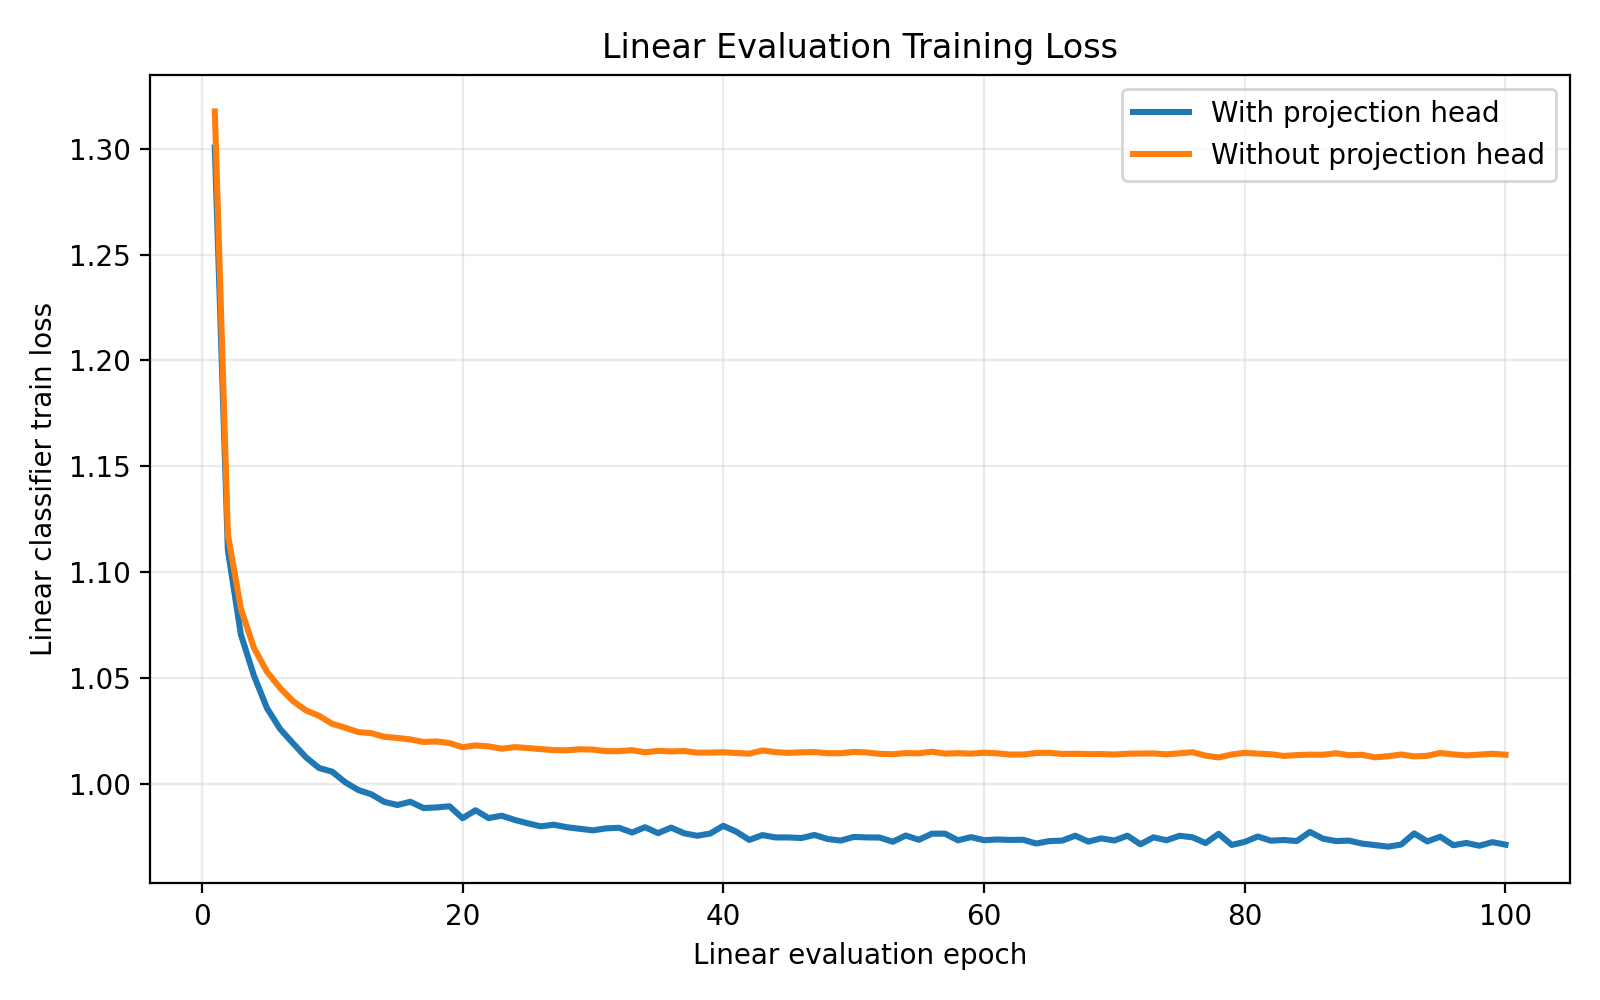
\includegraphics[width=\textwidth]{head_figures/loss_curve.png}
    \caption{Linear-evaluation loss.}
\end{subfigure}
\caption{Projection head ablation curves.}
\label{fig:projection-head}
\end{figure}

The projection head gives a modest improvement over the no-projection-head variant. This is consistent with the SimCLR design that applies the contrastive loss in the projected space $z$, while downstream evaluation uses the encoder feature $h$. Since the gain is small and not averaged over multiple seeds, we interpret it cautiously.


\subsection{Batch Size Ablation}
\label{sec:batch-size}

Batch size is important in SimCLR because it controls the number of in-batch negatives. With two views per image, each anchor has $2B-2$ negatives. Larger batches may provide more comparison samples and richer semantic diversity, but they also change the number of optimizer updates per epoch and may increase the probability of false negatives. We therefore compare batch sizes 128, 256, 512, and 1024 within the same controlled ablation group.

\begin{table}[H]
\centering
\small
\begin{tabular}{ccccc}
\toprule
\textbf{Batch size} & \textbf{Negatives/anchor} & \textbf{Best acc. (\%)} & \textbf{Best epoch} & \textbf{Final acc. (\%)} \\
\midrule
128 & 254 & 62.54 & 49 & 62.10 \\
256 & 510 & \textbf{63.47} & 29 & \textbf{63.33} \\
512 & 1022 & 60.89 & 45 & 60.29 \\
1024 & 2046 & 57.56 & 64 & 56.88 \\
\bottomrule
\end{tabular}
\caption{Linear evaluation result for the batch size ablation.}
\label{tab:batch-size}
\end{table}

\begin{figure}[H]
\centering
\begin{subfigure}{0.45\textwidth}
    \centering
    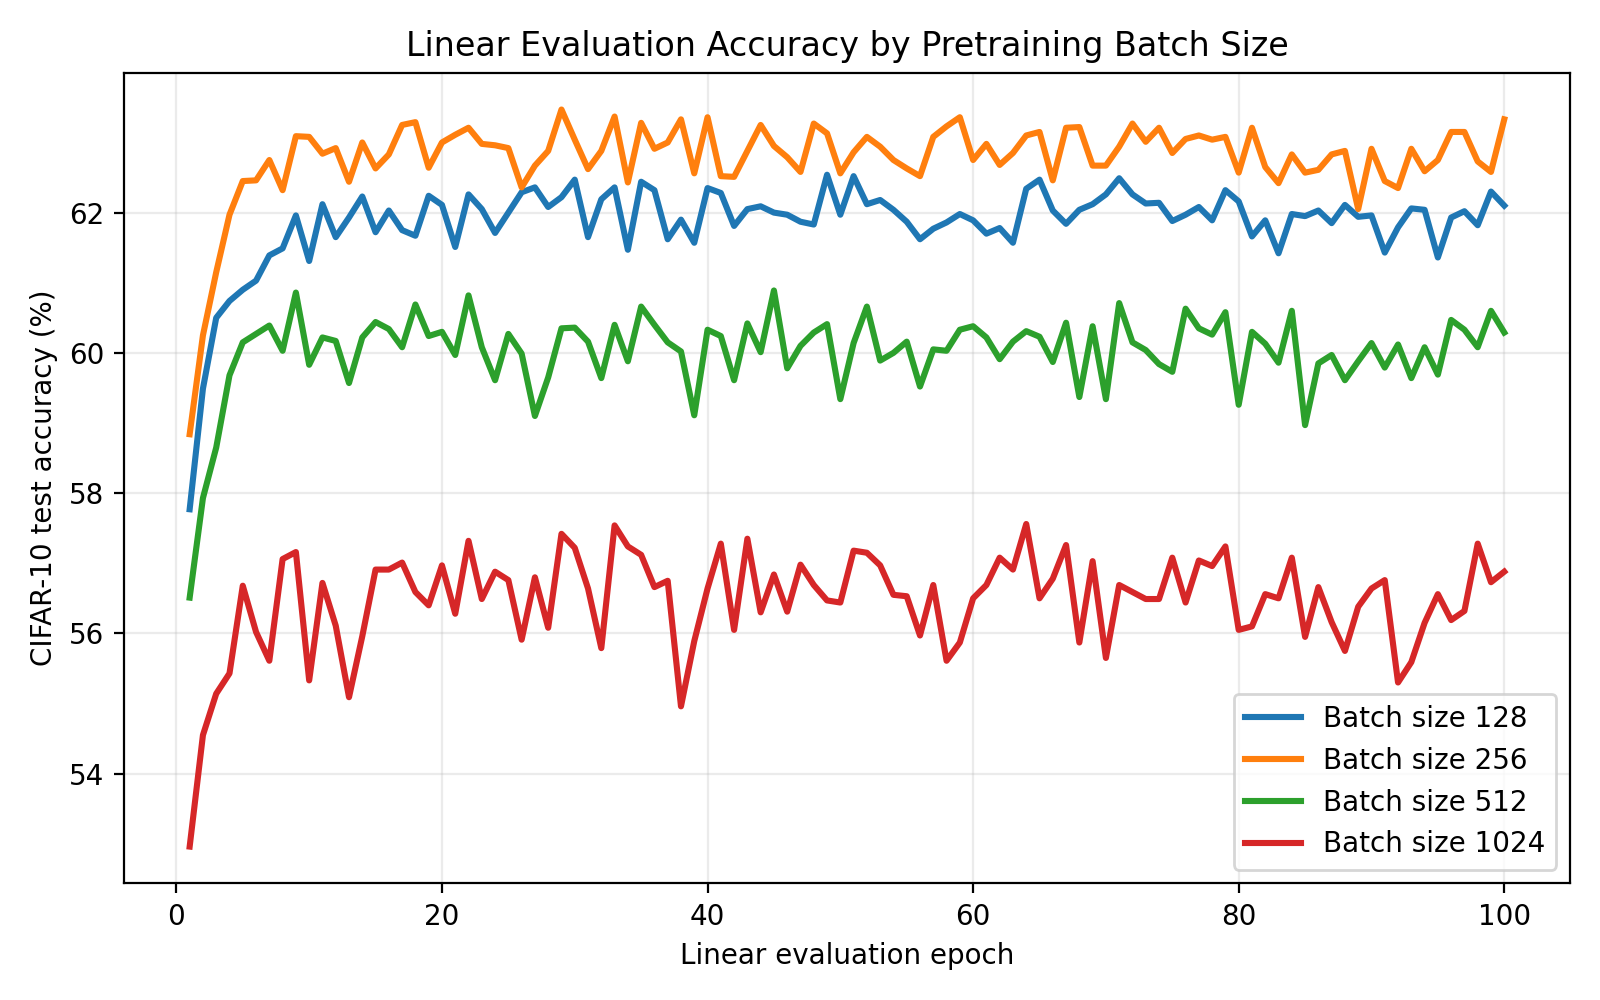
\includegraphics[width=\textwidth]{batch_figures/accuracy_curve.png}
    \caption{Linear-evaluation accuracy over epochs.}
\end{subfigure}
\hfill
\begin{subfigure}{0.45\textwidth}
    \centering
    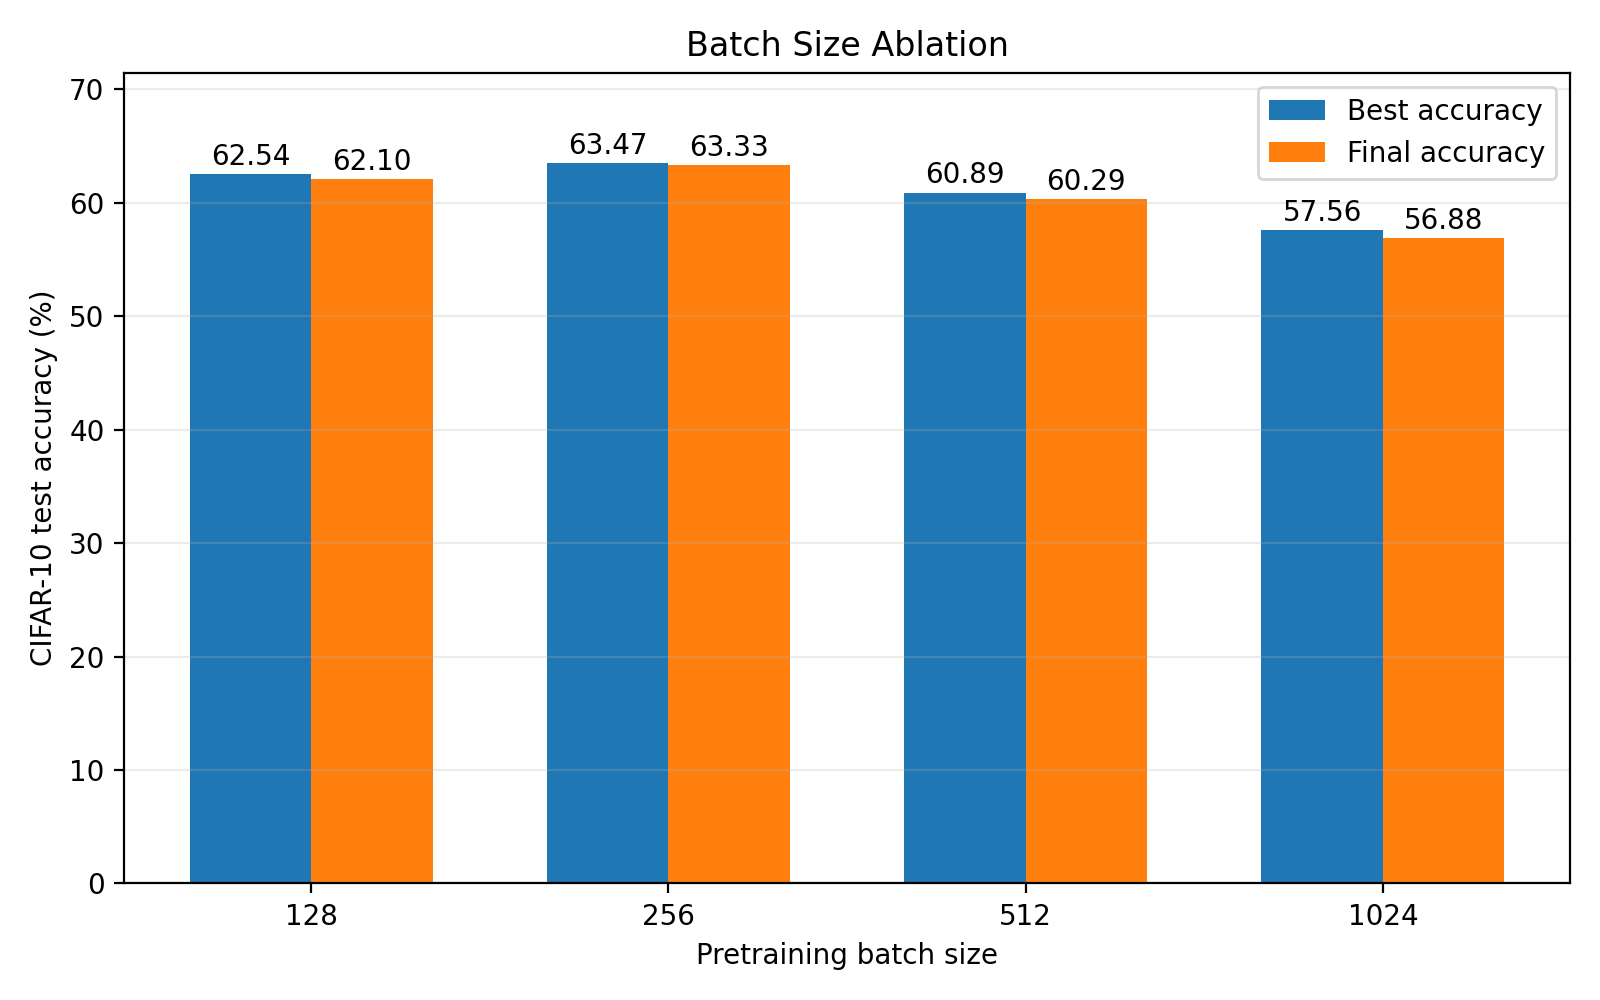
\includegraphics[width=\textwidth]{batch_figures/accuracy_bar.png}
    \caption{Best and final test accuracy.}
\end{subfigure}
\caption{Batch size ablation results.}
\label{fig:batch-size}
\end{figure}

The best result is obtained at batch size 256. Larger batches do not improve performance monotonically: batch sizes 512 and 1024 perform worse under the default training setup. This is interesting because larger batches provide more in-batch negatives, which could in principle help contrastive learning.

However, batch size changes more than the number of negatives. Under a fixed number of epochs, larger batches receive fewer optimizer updates. They may also introduce more false negatives, especially on CIFAR-10 with only ten classes. Therefore, the weaker large-batch results may reflect optimization mismatch or false negatives rather than the effect of negative-sample count alone. We test the optimization explanation with a learning-rate follow-up in Section~\ref{sec:lr-followup}.

\subsection{Low-Label Evaluation}

This experiment tests whether SimCLR representations are useful when only a small number of labels are available. We compare frozen linear evaluation, SimCLR initialization with fine-tuning, and supervised training from scratch. Since fine-tuning and supervised-from-scratch results were collected at 1\%, 10\%, and 100\% labels, the main comparison table reports these shared label fractions.

\begin{table}[H]
\centering
\small
\begin{tabular}{lccc}
\toprule
\textbf{Method / Evaluation Setting} & \textbf{1\%} & \textbf{10\%} & \textbf{100\%} \\
\midrule
Frozen SimCLR + Linear Classifier & 54.3 & 64.4 & 68.2 \\
SimCLR Init + Fine-tuning & \textbf{54.3} & \textbf{66.7} & \textbf{78.4} \\
Supervised From Scratch & 34.3 & 55.7 & 76.4 \\
\bottomrule
\end{tabular}
\caption{Label efficiency comparison under shared label fractions.}
\label{tab:low-label-combined}
\end{table}

The frozen linear evaluation also reaches 67.2\% with 50\% labels and 67.7\% with 80\% labels, showing that the frozen representation gradually saturates as more labels are added.

\begin{figure}[H]
\centering
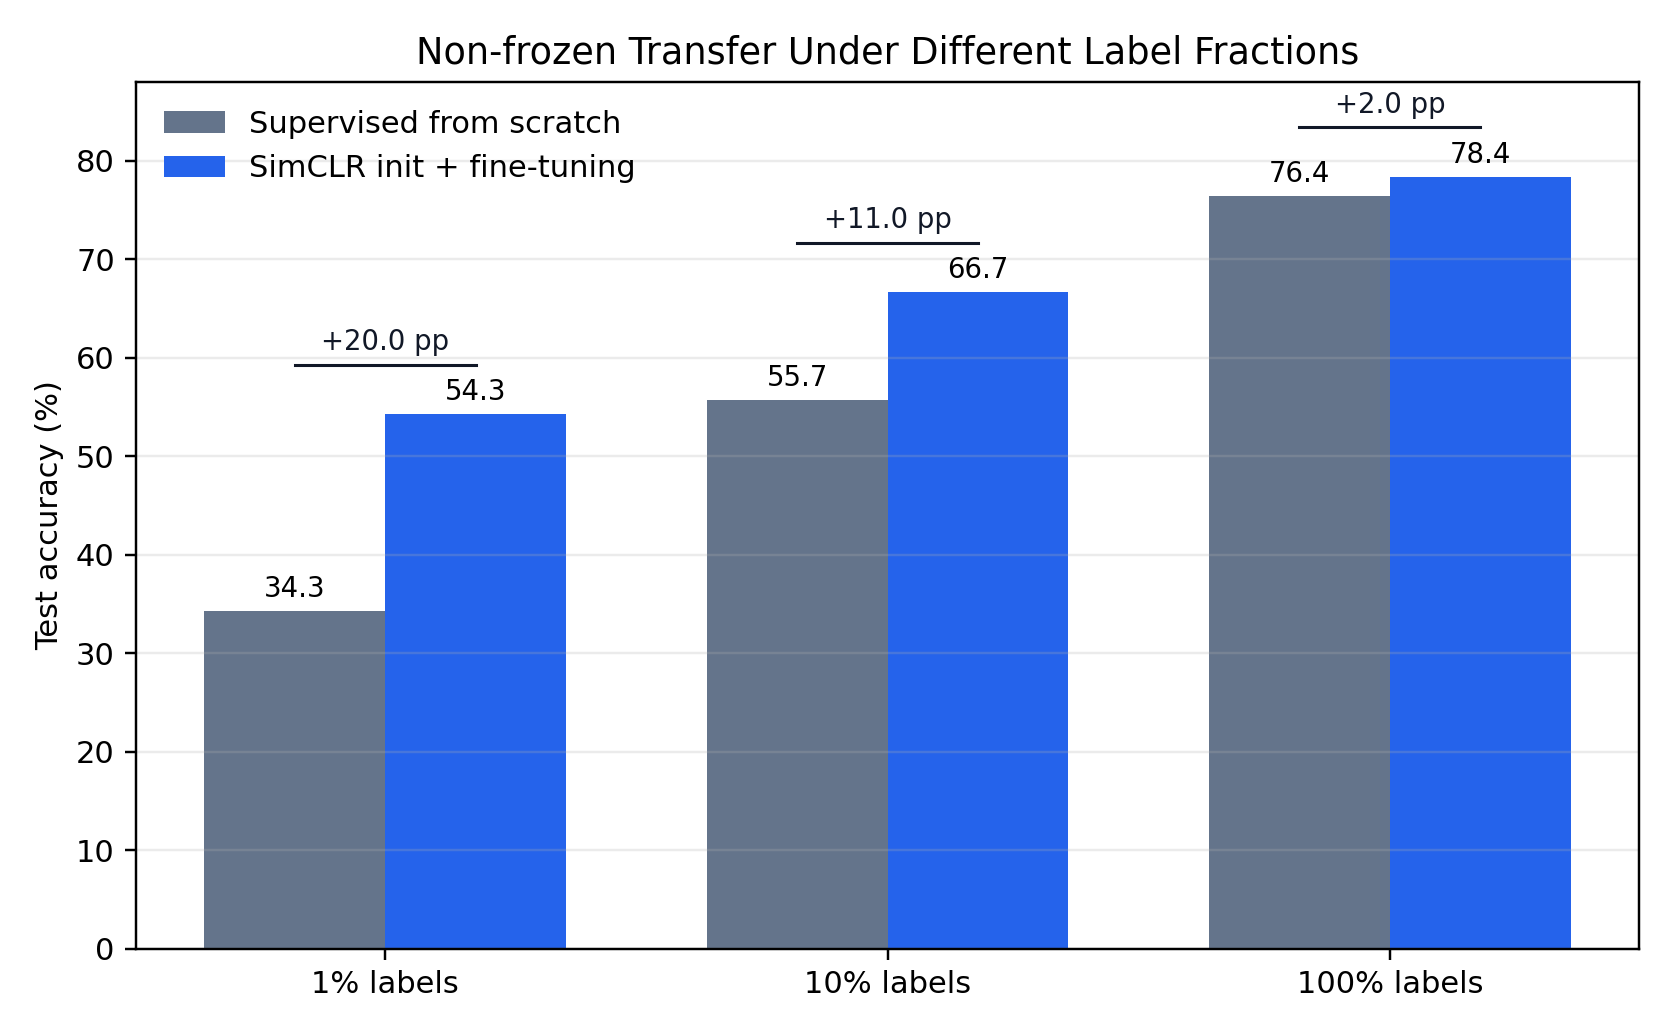
\includegraphics[width=0.60\textwidth]{low_label_figures/low_label_transfer_accuracy.png}
\caption{Non-frozen transfer accuracy under different label fractions.}
\label{fig:low-label-transfer}
\end{figure}

The frozen SimCLR features remain useful even with limited labels. With 10\% labels, the frozen linear classifier reaches 64.4\%, only 3.8 percentage points below the full-label frozen result. In the non-frozen transfer setting, SimCLR initialization gives the largest gain when labels are scarce: +20.0 percentage points at 1\% labels and +11.0 percentage points at 10\% labels. With all labels, the gain shrinks to 2.0 percentage points. This indicates that SimCLR mainly improves label efficiency rather than simply increasing fully supervised performance.

\subsection{Large-Batch Learning Rate Follow-up}
\label{sec:lr-followup}

The batch size ablation in Section~\ref{sec:batch-size} shows that batch size 1024 performs poorly under the default learning rate. This follow-up experiment checks whether the weak large-batch result is partly an optimization issue. We keep the batch size fixed at 1024 and sweep the pretraining learning rate.

\begin{table}[H]
\centering
\small
\begin{tabular}{lcc}
\toprule
\textbf{Learning rate} & \textbf{Best acc. (\%)} & \textbf{Change from default} \\
\midrule
$3 \times 10^{-4}$ & 57.56 & -- \\
$6 \times 10^{-4}$ & 63.73 & +6.17 \\
$1.2 \times 10^{-3}$ & \textbf{65.43} & +7.87 \\
$2.4 \times 10^{-3}$ & 61.22 & +3.66 \\
\bottomrule
\end{tabular}
\caption{Learning-rate sweep for batch size 1024.}
\label{tab:large-batch-lr}
\end{table}

\begin{figure}[H]
\centering
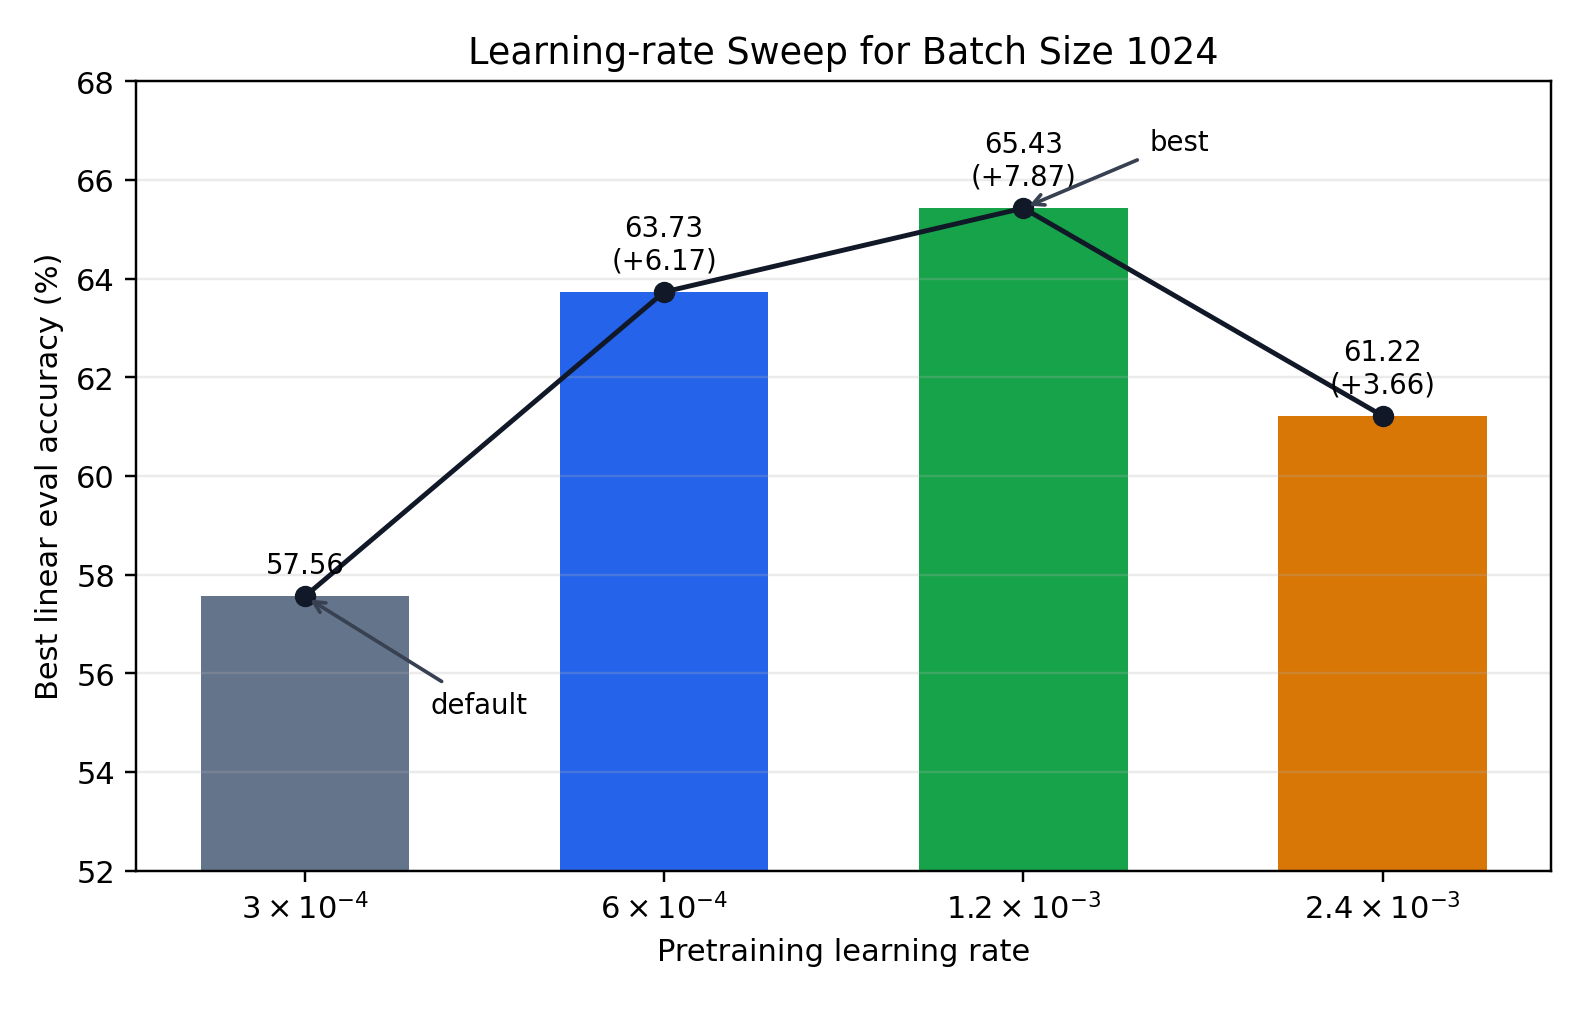
\includegraphics[width=0.70\textwidth]{lr_figures/large_batch_lr_sweep.png}
\caption{Learning-rate sweep for batch size 1024.}
\label{fig:large-batch-lr}
\end{figure}

The best result is obtained with learning rate $1.2 \times 10^{-3}$, improving the batch size 1024 result from 57.56\% to 65.43\%. This changes how we interpret the batch-size ablation: the weak default result does not mean that more negatives are always harmful. Instead, it suggests that large-batch SimCLR needs matched optimization. However, the drop at $2.4 \times 10^{-3}$ shows that simply increasing the learning rate is not always beneficial.

\section{Discussion}
\label{sec:discussion}

The ablations show that SimCLR performance is shaped by both representation design and optimization matching. Data augmentation and the projection head affect what information is preserved in the learned representation, while batch size and learning rate affect how effectively the contrastive objective is optimized.

\paragraph{Data Augmentation Shortcuts.}
The augmentation results show that ColorJitter is the most important tested augmentation. Removing it reduces frozen linear accuracy from 68.20\% to 62.61\%, even though the contrastive Top-1 score increases to 82.00\%. This mismatch suggests that the contrastive pretraining metric can become easier for the wrong reason. Without color perturbation, two views of the same image may preserve similar color statistics, allowing the encoder to match positive pairs through low-level shortcuts rather than learning more transferable semantic structure. In contrast, removing Gaussian blur has almost no effect, with linear accuracy remaining at 68.05\%. Since CIFAR-10 images are only $32 \times 32$ pixels, the images already contain limited high-frequency detail, so blur may add little useful invariance in this setting. These results support using frozen linear evaluation, rather than contrastive Top-1 alone, as the main measure of representation quality.

\paragraph{Projection Head.}
The projection head gives a modest but consistent improvement, increasing best linear evaluation accuracy from 62.16\% to 63.59\%. This is consistent with the SimCLR design, where the contrastive loss is applied to the projected representation $z$ while downstream evaluation uses the encoder feature $h$. A plausible explanation is that the projection head separates instance-level contrastive constraints from the representation used for classification. If NT-Xent is applied directly to $h$, some information useful for downstream class separation may be suppressed. The projection head therefore allows $z$ to absorb more of the contrastive objective, while $h$ may retain more general visual features. Since the gain is small and not averaged over multiple seeds, we interpret this result as supportive rather than conclusive evidence.

\paragraph{Batch Size and Optimization.}
The batch-size results differ from the simple expectation that more in-batch negatives should always help. Under the default learning rate, performance peaks at batch size 256 with 63.47\% best accuracy, but drops to 60.89\% at batch size 512 and 57.56\% at batch size 1024. This non-monotonic trend suggests that batch size changes more than the number of negatives.

First, larger batches receive fewer optimizer updates under a fixed epoch budget. This can slow training progress unless the learning rate or schedule is adjusted. The learning-rate sweep supports this interpretation: increasing the learning rate for batch size 1024 from $3 \times 10^{-4}$ to $1.2 \times 10^{-3}$ improves accuracy from 57.56\% to 65.43\%. However, the drop to 61.22\% at $2.4 \times 10^{-3}$ shows that large-batch training requires careful tuning rather than simply increasing the learning rate.

Second, larger batches may increase the false-negative problem on CIFAR-10. Because the dataset has only ten coarse classes, a large batch is more likely to contain images from the same semantic class as the anchor. SimCLR still treats these images as negatives and pushes them apart in representation space, which can weaken same-class clustering and reduce downstream linear separability. The large-batch degradation is therefore best interpreted as a combined effect of fewer updates, learning-rate mismatch, and possible false negatives.

\paragraph{Label Efficiency.}
The low-label results show that SimCLR mainly improves label efficiency. In frozen evaluation, using only 10\% labels reaches 64.4\% accuracy, only 3.8 percentage points below the full-label frozen result of 68.2\%. In the non-frozen transfer setting, SimCLR initialization gives the largest benefit when labels are scarce: at 1\% labels, it improves accuracy from 34.3\% to 54.3\%, a gain of 20.0 percentage points. The gain decreases to 11.0 percentage points at 10\% labels and 2.0 percentage points at 100\% labels. This pattern suggests that contrastive pretraining is most useful when supervision is limited, while its advantage becomes smaller as labeled data becomes sufficient.

\section{Shortcomings}

There are several limitations in the current experiments. First, due to limited CPU-based computation time, we prioritized running a wider set of controlled ablations over repeating every setting with many independent random seeds. Although some settings were checked with repeated 100-epoch evaluation runs, we do not report full mean and standard deviation for every setting. Therefore, the results should not be interpreted as complete statistical estimates. Small differences, such as 68.20\% versus 68.05\%, should not be over-interpreted. Instead, our main conclusions rely on larger and more interpretable trends, such as the drop caused by removing ColorJitter, the recovery of batch size 1024 after learning-rate tuning, and the low-label gains from SimCLR initialization.

Second, when best accuracy is reported, it refers to the highest test accuracy observed during the corresponding 100-epoch linear evaluation, rather than an average over many random seeds. In addition, the experiments use CIFAR-10 and ResNet-18 only, so the conclusions may not transfer directly to larger datasets or architectures. Finally, some comparisons use the same number of epochs rather than the same number of optimization steps, which can disadvantage larger batches because they receive fewer optimizer updates.

\section{Future Work}

Future work could run each setting with multiple independent random seeds and report mean and standard deviation. The batch size ablation could be extended with learning-rate scaling, longer pretraining, LARS or SGD with momentum, temperature tuning, and schedules matched by optimization steps rather than epochs. Additional k-nearest-neighbor evaluation and visualization of feature space could help explain how different ablations change the learned representation space. Finally, testing larger datasets or deeper backbones would show whether the observed trends transfer beyond CIFAR-10 and ResNet-18.

\section{Conclusion}

This project presents a controlled ablation study of SimCLR on CIFAR-10 using a ResNet-18 encoder. Removing ColorJitter causes the largest drop in downstream accuracy, even though it achieves the highest contrastive Top-1 score, showing that pretraining metrics do not always reflect downstream representation quality. The projection head gives a modest improvement in linear evaluation accuracy, consistent with the SimCLR design of learning in a separate projected space. In the batch size experiments, batch size 256 performs best under the default settings, but batch size 1024 improves to 65.43\% when the learning rate is matched, suggesting that large-batch performance depends strongly on optimization settings. Finally, the low-label experiments show that SimCLR mainly improves label efficiency, with the largest gain at 1\% labels. Overall, SimCLR works well in our lightweight setting, but its performance is affected by augmentation design, projection head usage, and optimization matching.

\begin{thebibliography}{10}

\bibitem{sthalles_simclr}
T. Silva.
\textit{PyTorch SimCLR: A Simple Framework for Contrastive Learning of Visual Representations}.
GitHub repository, 2020.
\url{https://github.com/sthalles/SimCLR}


\bibitem{simclr}
T. Chen, S. Kornblith, M. Norouzi, and G. Hinton.
\textit{A Simple Framework for Contrastive Learning of Visual Representations}.
ICML, 2020.
\url{https://arxiv.org/abs/2002.05709}


\bibitem{cpc}
A. van den Oord, Y. Li, and O. Vinyals.
\textit{Representation Learning with Contrastive Predictive Coding}.
arXiv preprint arXiv:1807.03748, 2018.
\url{https://arxiv.org/abs/1807.03748}

\bibitem{moco}
K. He, H. Fan, Y. Wu, S. Xie, and R. Girshick.
\textit{Momentum Contrast for Unsupervised Visual Representation Learning}.
CVPR, 2020.
\url{https://arxiv.org/abs/1911.05722}

\bibitem{goodviews}
Y. Tian, C. Sun, B. Poole, D. Krishnan, C. Schmid, and P. Isola.
\textit{What Makes for Good Views for Contrastive Learning?}
NeurIPS, 2020.
\url{https://arxiv.org/abs/2005.10243}

\bibitem{alignuniform}
T. Wang and P. Isola.
\textit{Understanding Contrastive Representation Learning through Alignment and Uniformity on the Hypersphere}.
ICML, 2020.
\url{https://arxiv.org/abs/2005.10242}

\bibitem{simclrv2}
T. Chen, S. Kornblith, K. Swersky, M. Norouzi, and G. Hinton.
\textit{Big Self-Supervised Models are Strong Semi-Supervised Learners}.
NeurIPS, 2020.
\url{https://arxiv.org/abs/2006.10029}

\bibitem{supcon}
P. Khosla, P. Teterwak, C. Wang, A. Sarna, Y. Tian, P. Isola, A. Maschinot, C. Liu, and D. Krishnan.
\textit{Supervised Contrastive Learning}.
NeurIPS, 2020.
\url{https://arxiv.org/abs/2004.11362}

\bibitem{cifar10}
A. Krizhevsky.
\textit{Learning Multiple Layers of Features from Tiny Images}.
Technical report, 2009.
\url{https://www.cs.toronto.edu/~kriz/cifar.html}

\bibitem{resnet}
K. He, X. Zhang, S. Ren, and J. Sun.
\textit{Deep Residual Learning for Image Recognition}.
CVPR, 2016.
\url{https://arxiv.org/abs/1512.03385}

\end{thebibliography}

\end{document}